\documentclass{beamer}
\usetheme{Madrid}
\usecolortheme{default}

\usepackage{amsmath, amssymb}
\usepackage{enumerate}
\usepackage{graphicx}
\usepackage{listings}
\usepackage{tcolorbox}
\tcbuselibrary{listings, skins}

\newtcblisting{mycode}{
  arc=0mm,
  boxrule=0.5pt,
  colback=white,
  colframe=black,
  listing only,
  listing options={
    language=Python,
    basicstyle=\small\ttfamily,
    keywordstyle=\color{blue},
    commentstyle=\color{blue},
    stringstyle=\color{red},
    showstringspaces=false,
    breaklines=true
  },
  sharp corners,
  enhanced,
}

\lstset{
  language=Python,
  basicstyle=\ttfamily\small,
  keywordstyle=\bfseries,
  showstringspaces=false,
  breaklines=true
}

\title{Analog-1.1.44}
\author{SAI HASINI PAPPULA-EE25BTECH11044}
\date{\today}

% ─────────────────────────────────────────────────────────────────────────────
\begin{document}

\begin{frame}
  \titlepage
\end{frame}

% ─── Problem Statement ───────────────────────────────────────────────────────
\begin{frame}{Problem}
\textbf{A signal is processed by a causal filter with transfer function $G(s)$.}

\vspace{0.8em}
For a \textbf{distortion-free output waveform}, $G(s)$ must:

\vspace{0.5em}
\begin{enumerate}[(a)]
  \item Provide zero phase shift for all frequencies
  \item Provide constant phase shift for all frequencies
  \item Provide linear phase shift proportional to frequency
  \item Provide phase shift inversely proportional to frequency
\end{enumerate}
\end{frame}

% ─── Core Concept ────────────────────────────────────────────────────────────
\begin{frame}{What is a Distortion-Free System?}
A system is \textbf{distortion-free} if the output is a scaled and time-delayed
replica of the input:
\[
  y(t) = K\,x(t - t_0), \qquad K > 0,\; t_0 \geq 0
\]

\vspace{0.5em}
\begin{block}{Interpretation}
\begin{itemize}
  \item $K$ — uniform scaling (amplitude change only, no shape distortion)
  \item $t_0$ — uniform time delay (all frequency components delayed equally)
\end{itemize}
\end{block}

\vspace{0.5em}
Taking the Fourier transform of $y(t) = K\,x(t-t_0)$:
\[
  Y(j\omega) = K\,e^{-j\omega t_0}\,X(j\omega)
\]
\[
  \therefore\quad G(j\omega) \;=\; K\,e^{-j\omega t_0}
\]
\end{frame}

% ─── Fourier Transform Solution ──────────────────────────────────────────────
\begin{frame}{Fourier Transform Approach}
\textbf{Step 1:} Express the input as a sum of sinusoids (Fourier series/transform):
\[
  x(t) = \sum_{n} A_n \cos(\omega_n t + \phi_n)
\]

\textbf{Step 2:} Each component passes through $G(j\omega)$:
\[
  |G(j\omega_n)| = K, \qquad \angle G(j\omega_n) = -\omega_n t_0
\]

\textbf{Step 3:} Output of each component:
\[
  y_n(t) = K \cdot A_n \cos\!\left(\omega_n t + \phi_n - \omega_n t_0\right)
         = K \cdot A_n \cos\!\left(\omega_n(t - t_0) + \phi_n\right)
\]

\textbf{Step 4:} Superposition gives:
\[
  y(t) = \sum_n y_n(t) = K\,x(t - t_0) \checkmark
\]

Every component is delayed by the \emph{same} $t_0$ — shape preserved.
\end{frame}

% ─── Required Conditions ─────────────────────────────────────────────────────
\begin{frame}{Required Conditions on $G(j\omega)$}
From $G(j\omega) = K\,e^{-j\omega t_0}$, two conditions follow:

\vspace{0.4em}
\textbf{Condition 1 — Magnitude (Flat):}
\[
  \bigl|G(j\omega)\bigr| = K \quad (\text{constant for all }\omega)
\]

\vspace{0.4em}
\textbf{Condition 2 — Phase (Linear):}
\[
  \angle G(j\omega) = -\omega t_0 \quad (\text{linear in }\omega)
\]

\vspace{0.5em}
\begin{block}{Group Delay}
The group delay must be constant:
\[
  \tau_g(\omega) = -\frac{d}{d\omega}\angle G(j\omega) = t_0 = \text{const}
\]
Constant group delay $\Leftrightarrow$ linear phase $\Leftrightarrow$ no phase distortion.
\end{block}
\end{frame}

% ─── Example 1 ───────────────────────────────────────────────────────────────
\begin{frame}{Example 1: Two-Component Signal}
Let $x(t) = \cos(2\pi t) + \cos(6\pi t)$, with $K = 1$, $t_0 = 0.5\,$s.

\vspace{0.5em}
\textbf{Fourier analysis:} Two components at $\omega_1 = 2\pi$ and $\omega_2 = 6\pi$.

\vspace{0.3em}
\textbf{Phase applied by $G(j\omega) = e^{-j\omega t_0}$:}
\[
  \angle G(j\omega_1) = -2\pi \times 0.5 = -\pi \;\text{ rad}
\]
\[
  \angle G(j\omega_2) = -6\pi \times 0.5 = -3\pi \;\text{ rad}
\]

\textbf{Output:}
\[
  y(t) = \cos(2\pi(t-0.5)) + \cos(6\pi(t-0.5))
       = \cos(2\pi t - \pi) + \cos(6\pi t - 3\pi)
\]
\[
  = x(t - 0.5) \checkmark
\]
\begin{block}{Observation}
Both components delayed by the same $t_0 = 0.5\,$s. Output shape = input shape.
\end{block}
\end{frame}

% ─── Example 2 ───────────────────────────────────────────────────────────────
\begin{frame}{Example 2: Constant Phase (Non-Distortion-Free)}
Let $x(t) = \cos(2\pi t) + \cos(6\pi t)$, but now $\angle G(j\omega) = -\dfrac{\pi}{2}$ (constant).

\vspace{0.5em}
\textbf{Time delay per component:}
\[
  t_{\text{delay}}(\omega_1) = \frac{\pi/2}{2\pi} = 0.25\;\text{s}
\]
\[
  t_{\text{delay}}(\omega_2) = \frac{\pi/2}{6\pi} = 0.083\;\text{s}
\]

\textbf{Output:}
\[
  y(t) = \cos(2\pi t - \tfrac{\pi}{2}) + \cos(6\pi t - \tfrac{\pi}{2})
\]
\[
  = \cos\!\bigl(2\pi(t-0.25)\bigr) + \cos\!\bigl(6\pi(t-0.083)\bigr)
\]

\begin{block}{Observation}
Different delays for different frequencies $\Rightarrow$ shape changes $\Rightarrow$ \textbf{distortion}.
\end{block}
\end{frame}

% ─── Example 3 ───────────────────────────────────────────────────────────────
\begin{frame}{Example 3: Linear Phase Verified Numerically}
$x(t) = \cos(2\pi t) + 0.4\cos(6\pi t) + 0.2\cos(10\pi t)$, $K=0.6$, $t_0=0.3\,$s.

\vspace{0.3em}
\textbf{Phase at each frequency:}

\vspace{0.2em}
\begin{center}
\renewcommand{\arraystretch}{1.4}
\begin{tabular}{|c|c|c|c|}
\hline
$\omega$ (rad/s) & $\angle G = -\omega t_0$ & $t_{\text{delay}}$ & Distortion? \\
\hline
$2\pi \approx 6.28$ & $-1.885$ rad & $0.3\,$s & No \\
$6\pi \approx 18.85$ & $-5.655$ rad & $0.3\,$s & No \\
$10\pi \approx 31.42$ & $-9.425$ rad & $0.3\,$s & No \\
\hline
\end{tabular}
\end{center}

\vspace{0.4em}
\begin{block}{Observation}
All three components have identical delay $t_0 = 0.3\,$s. \\
$y(t) = 0.6\,x(t - 0.3)$ — distortion-free. $\checkmark$
\end{block}
\end{frame}

% ─── Option (a) ──────────────────────────────────────────────────────────────
\begin{frame}{Option (a): Zero Phase Shift}

\textbf{Claim:} $\angle G(j\omega) = 0$ for all $\omega$.

\vspace{0.5em}
This means $G(j\omega) = K$ (purely real), implying:
\[
  t_0 = 0 \quad \Longrightarrow \quad y(t) = K\,x(t)
\]

\vspace{0.4em}
\textbf{Problems:}
\begin{itemize}
  \item Zero delay requires the filter to be \textbf{non-causal} — the output
        responds instantaneously at all frequencies, which is physically
        unrealisable for a real causal system.
  \item It is an overly restrictive special case ($t_0 = 0$). Distortion-free
        transmission is possible with $t_0 > 0$.
\end{itemize}

\vspace{0.4em}
\begin{block}{Conclusion}
  Option (a) is \textbf{incorrect}.
\end{block}
\end{frame}

% ─── Option (b) ──────────────────────────────────────────────────────────────
\begin{frame}{Option (b): Constant Phase Shift}

\textbf{Claim:} $\angle G(j\omega) = -\phi_0$ (a fixed constant) for all $\omega$.

\vspace{0.5em}
The time delay experienced by frequency component $\omega$ is:
\[
  t_{\text{delay}}(\omega) = \frac{\phi_0}{\omega}
\]
This \textbf{varies with frequency} — low-frequency components are delayed more
than high-frequency ones.

\vspace{0.4em}
\textbf{Numerical example} ($\phi_0 = \pi/2$):
\[
  \omega = 2\pi\;\text{rad/s}:\; t_0 = 0.25\;\text{s}
  \qquad
  \omega = 4\pi\;\text{rad/s}:\; t_0 = 0.125\;\text{s}
\]
Different delays $\Rightarrow$ waveform shape changes $\Rightarrow$ distortion.

\vspace{0.4em}
\begin{block}{Conclusion}
  Option (b) is \textbf{incorrect}.
\end{block}
\end{frame}

% ─── Option (c) ──────────────────────────────────────────────────────────────
\begin{frame}{Option (c): Linear Phase Proportional to Frequency}

\textbf{Claim:} $\angle G(j\omega) = -\omega t_0$ (linear in $\omega$).

\vspace{0.5em}
Time delay for frequency $\omega$:
\[
  t_{\text{delay}}(\omega) = \frac{\omega t_0}{\omega} = t_0 \quad (\text{constant!})
\]

Every frequency component is delayed by the \emph{same} $t_0$ seconds, so the
output waveform is identical in shape to the input:
\[
  y(t) = K\,x(t-t_0) \checkmark
\]

Group delay: $\tau_g = t_0 = \text{const}\ \checkmark$

\vspace{0.4em}
\begin{block}{Conclusion}
  Option (c) is \textbf{correct}. Linear phase is the necessary and sufficient
  phase condition for distortion-free transmission.
\end{block}
\end{frame}

% ─── Option (d) ──────────────────────────────────────────────────────────────
\begin{frame}{Option (d): Phase Inversely Proportional to Frequency}

\textbf{Claim:} $\displaystyle\angle G(j\omega) = \frac{-K}{\omega}$.

\vspace{0.5em}
Time delay:
\[
  t_{\text{delay}}(\omega) = \frac{K/\omega}{\omega} = \frac{K}{\omega^2}
  \quad \Longrightarrow \quad \text{frequency-dependent delay}
\]

Group delay:
\[
  \tau_g(\omega) = -\frac{d}{d\omega}\!\left(\frac{-K}{\omega}\right)
                = \frac{K}{\omega^2} \neq \text{const}
\]

Non-constant group delay $\Rightarrow$ phase distortion.

\vspace{0.4em}
\begin{block}{Conclusion}
  Option (d) is \textbf{incorrect}.
\end{block}
\end{frame}

% ─── Summary Table ───────────────────────────────────────────────────────────
\begin{frame}{Summary}

\begin{center}
\renewcommand{\arraystretch}{1.6}
\begin{tabular}{clccc}
\hline
\textbf{Option} & \textbf{Phase} $\angle G(j\omega)$
  & \textbf{Delay} $t_d(\omega)$
  & \textbf{Group Delay}
  & \textbf{Verdict} \\
\hline
(a) & $0$ & $0$ (non-causal) & $0$ & Incorrect \\
(b) & $-\phi_0$ (const) & $\phi_0/\omega$ & varies & Incorrect \\
(c) & $-\omega t_0$ (linear) & $t_0$ & $t_0$ = const & \textbf{Correct} \\
(d) & $-K/\omega$ & $K/\omega^2$ & varies & Incorrect \\
\hline
\end{tabular}
\end{center}

\vspace{0.6em}
\begin{block}{Answer}
\textbf{Option (c)} — Linear phase $\angle G(j\omega) = -\omega t_0$ ensures
all frequency components experience the same time delay, giving
$y(t) = K\,x(t - t_0)$.
\end{block}
\end{frame}

% ─── Python Code (Part 1) ────────────────────────────────────────────────────
\begin{frame}[fragile]
\frametitle{Python Code for Plot}
\begin{mycode}
import numpy as np
import matplotlib.pyplot as plt

# Time axis
t = np.linspace(0, 4, 1000)

# Parameters: scale factor and time delay
K  = 0.6
t0 = 0.5

# Input signal (composite of two sinusoids)
x = np.sin(2*np.pi*t) + 0.4*np.sin(2*np.pi*3*t)

\end{mycode}
\end{frame}

% ─── Python Code (Part 2) ────────────────────────────────────────────────────
\begin{frame}[fragile]
\frametitle{Python Code for Plot}
\begin{mycode}
# Distortion-free output: scaled and delayed
y = K*(np.sin(2*np.pi*(t-t0)) + 0.4*np.sin(2*np.pi*3*(t-t0)))

plt.figure(figsize=(8, 3.5))
plt.plot(t, x, 'b-',  linewidth=1.8, label=r'Input $x(t)$')
plt.plot(t, y, 'r--', linewidth=1.8,
         label=r'Output $y(t)=K\,x(t-t_0)$')

# Annotate the time delay
plt.annotate('', xy=(0.5+t0, 0.95), xytext=(0.5, 0.95),
             arrowprops=dict(arrowstyle='<->', color='black'))

\end{mycode}
\end{frame}

% ─── Python Code (Part 3) ────────────────────────────────────────────────────
\begin{frame}[fragile]
\frametitle{Python Code for Plot}
\begin{mycode}

plt.text(0.63, 1.0, r'$t_0=0.5\,$s', fontsize=9)
plt.xlabel(r'$t$ (s)'); 
plt.ylabel('Amplitude')
plt.title(r'Distortion-Free Output: $K=0.6$, $t_0=0.5\,$s')

plt.legend();
plt.grid(True, linestyle='--', alpha=0.5)
plt.tight_layout(); 

plt.savefig('plot1.png', dpi=150)

\end{mycode}
\end{frame}

% ─── Plot Frame ──────────────────────────────────────────────────────────────
\begin{frame}{Plot: Distortion-Free Output}
\begin{center}
  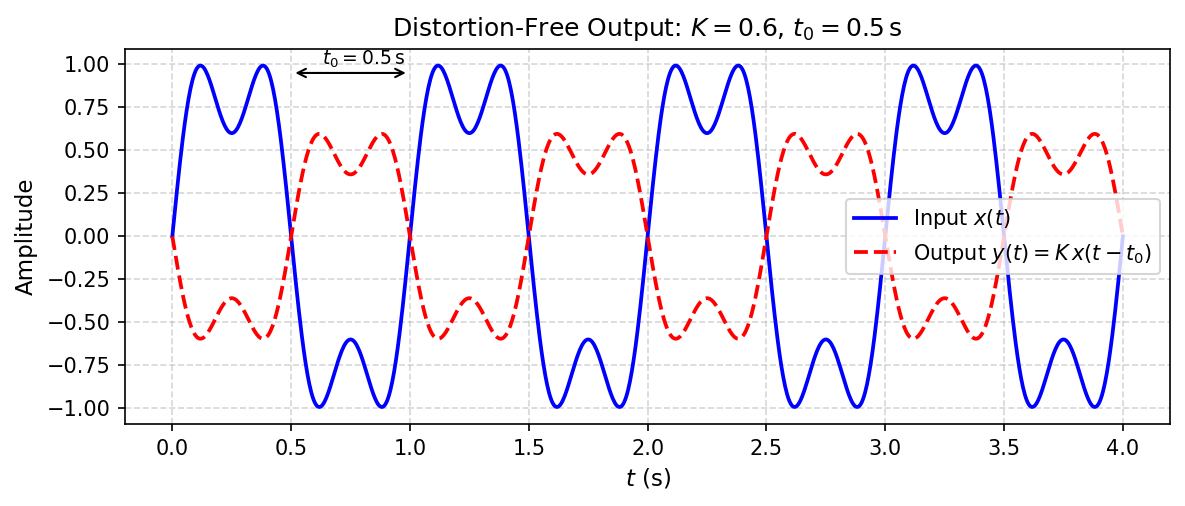
\includegraphics[width=0.95\textwidth]{plot1.png}
\end{center}
\begin{itemize}
  \item Output has the \textbf{same shape} as the input — no distortion.
  \item Amplitude is scaled by $K = 0.6$ and signal is shifted right by $t_0 = 0.5\,$s.
\end{itemize}
\end{frame}

\end{document}